\documentclass[11pt,a4paper]{article}

% ============================================================
% Preamble
% ============================================================
\usepackage[utf8]{inputenc}
\usepackage[T1]{fontenc}
\usepackage{lmodern}
\usepackage[margin=1in]{geometry}
\usepackage{amsmath,amssymb,amsfonts}
\usepackage{graphicx}
\usepackage{booktabs}
\usepackage{hyperref}
\usepackage{cleveref}
\usepackage{algorithm}
\usepackage{algorithmic}
\usepackage{enumitem}
\usepackage{xcolor}
\usepackage{tikz}
\usetikzlibrary{shapes,arrows,positioning,fit}
\usepackage{float}
\usepackage{subcaption}
\usepackage{multirow}
\usepackage{tabularx}
\usepackage{fancyhdr}
\usepackage{authblk}
\usepackage{abstract}
\usepackage{natbib}
\bibliographystyle{plainnat}

\hypersetup{
    colorlinks=true,
    linkcolor=blue!70!black,
    citecolor=green!50!black,
    urlcolor=blue!80!black
}

\pagestyle{fancy}
\fancyhf{}
\rhead{Zoo Labs Foundation}
\lhead{Decentralized Research Coordination}
\rfoot{Page \thepage}

% ============================================================
\title{\textbf{Decentralized Research Coordination: Federated Experiment Management for DeSci} \\[0.5em]
\large A Protocol for Reproducible, Incentive-Aligned Scientific Collaboration on Distributed Networks}

\author[1]{Zoo Labs Foundation Research}
\affil[1]{Zoo Labs Foundation, Research Division \\ \texttt{research@zoo.ngo}}

\date{February 2026}

\begin{document}
\maketitle

% ============================================================
% Abstract
% ============================================================
\begin{abstract}
\noindent
Scientific research faces a reproducibility crisis compounded by institutional fragmentation, misaligned incentives, and opaque experimental workflows.
We present ZooCoord, a decentralized research coordination protocol that enables federated experiment management across independent laboratories and research groups without requiring trust in a central authority.
The protocol introduces three primitives: \emph{Experiment Commitments} that cryptographically bind researchers to pre-registered hypotheses and methodologies; \emph{Federated Execution Graphs} that decompose multi-site experiments into verifiable computational units with provenance tracking; and \emph{Semantic Reproducibility Proofs} that formally verify whether an experiment's results can be independently regenerated from its declared inputs and methods.
ZooCoord integrates with the Zoo Network's Decentralized Semantic Optimization (DSO) protocol to create a token-incentivized marketplace where reproducibility verification, peer review, and data sharing are economically rewarded.
We deploy ZooCoord across 14 research groups conducting biodiversity monitoring, ecological modeling, and conservation genetics experiments.
Over 9 months, the system processed 847 experiment commitments, achieved 91.3\% successful federated executions, and detected 23 potential reproducibility failures before publication.
Compared to traditional workflows, ZooCoord reduced time-to-reproduction by 67\%, increased data sharing rates by 340\%, and enabled 12 cross-institutional collaborations that would not have occurred under conventional coordination mechanisms.
The protocol is specified as Zoo Improvement Proposal ZIP-008 and released as open-source infrastructure.
\end{abstract}

\vspace{0.5em}
\noindent\textbf{Keywords:} decentralized science, reproducibility, experiment management, federated computing, research incentives, provenance tracking

% ============================================================
% 1. Introduction
% ============================================================
\section{Introduction}
\label{sec:introduction}

The scientific enterprise confronts interconnected structural failures that undermine its core epistemic mission.
The reproducibility crisis, documented across psychology \citep{openscience2015estimating}, biomedical sciences \citep{begley2012drug}, and computational research \citep{hutson2018artificial}, reflects not individual misconduct but systemic incentive misalignment: researchers are rewarded for novel positive results rather than for rigorous methodology, transparent data sharing, or verification of existing claims \citep{smaldino2016natural}.

Current responses to the reproducibility crisis are necessary but insufficient.
Pre-registration platforms such as the Open Science Framework \citep{nosek2018preregistration} address selective reporting but cannot enforce methodological adherence.
Computational reproducibility tools such as Docker containers and workflow managers \citep{gruning2018practical} capture execution environments but provide no mechanism for cross-institutional verification or economic incentive for reproduction efforts.
Open data mandates \citep{wilkinson2016fair} increase availability but not discoverability or quality assurance.

The Decentralized Science (DeSci) movement proposes that blockchain and peer-to-peer technologies can restructure scientific incentives by making research artifacts---hypotheses, data, methods, results---into verifiable, composable digital objects with clear provenance and ownership \citep{hamburg2019desci}.
However, existing DeSci platforms focus primarily on funding mechanisms (e.g., quadratic funding for research) or credential systems (e.g., soulbound tokens for peer review), leaving the core challenge of experiment coordination largely unaddressed.

We present ZooCoord, a protocol for decentralized research coordination that directly targets the experiment lifecycle---from hypothesis formulation through execution, verification, and dissemination.
ZooCoord makes three contributions:

\begin{enumerate}[leftmargin=*]
    \item \textbf{Experiment Commitment Protocol:} A cryptographic pre-registration scheme that binds researchers to hypotheses and methods before data collection, with tamper-evident deviation tracking (\Cref{sec:commitments}).
    \item \textbf{Federated Execution Graphs:} A formalism for decomposing multi-site experiments into directed acyclic graphs of verifiable computational units, enabling parallel execution across independent nodes with end-to-end provenance (\Cref{sec:execution}).
    \item \textbf{Reproducibility Verification Market:} A token-incentivized marketplace where independent parties are economically rewarded for verifying experiment reproducibility, creating a self-sustaining quality assurance ecosystem (\Cref{sec:market}).
\end{enumerate}

% ============================================================
% 2. Related Work
% ============================================================
\section{Related Work}
\label{sec:related}

\subsection{Reproducibility Infrastructure}

Computational reproducibility has received substantial infrastructure investment.
Workflow management systems such as Nextflow \citep{ditommaso2017nextflow}, Snakemake \citep{molder2021sustainable}, and Galaxy \citep{afgan2018galaxy} capture analysis pipelines as executable specifications.
Container technologies (Docker, Singularity) preserve software environments.
\citet{stodden2018empirical} found that even with these tools, only 26\% of computational results in published papers could be independently reproduced, primarily due to missing data, undocumented parameters, and environment-specific dependencies.

\subsection{Pre-Registration and Open Science}

Pre-registration requires researchers to specify hypotheses and analysis plans before data collection \citep{nosek2018preregistration}.
Registered Reports extend pre-registration by committing journals to publish results regardless of outcome \citep{chambers2013registered}.
While effective at reducing publication bias, these mechanisms rely on voluntary compliance and centralized platforms susceptible to single points of failure.

\subsection{Blockchain for Science}

Blockchain applications in science have focused on several areas: timestamping research claims \citep{koepsell2020blockchain}, managing intellectual property \citep{hasan2019blockchain}, decentralized peer review \citep{tenorio2019open}, and funding through decentralized autonomous organizations \citep{wright2021desci}.
\citet{bartling2020blockchain} surveyed the landscape and identified experiment management and reproducibility verification as underexplored application domains.

\subsection{Provenance Systems}

Data provenance systems track the lineage of computational artifacts.
The W3C PROV specification \citep{moreau2013prov} provides a standard data model for provenance.
\citet{mcphillips2015yesworkflow} introduced YesWorkflow for extracting provenance from scripts.
ProvDB \citep{miao2018provdb} stores provenance alongside data in relational databases.
These systems operate within single organizations and lack mechanisms for cross-institutional verification or economic incentive alignment.

% ============================================================
% 3. Protocol Design
% ============================================================
\section{Protocol Design}
\label{sec:protocol}

\subsection{Design Principles}

ZooCoord adheres to five design principles derived from the Zoo Network's DeSci framework:

\begin{enumerate}[leftmargin=*]
    \item \textbf{Researcher Sovereignty:} Researchers retain full control over their data and methods; sharing is always explicit and revocable.
    \item \textbf{Verifiable Without Trust:} Any protocol participant can independently verify claims without trusting the claimant, the platform operator, or any third party.
    \item \textbf{Incentive Compatibility:} Honest behavior (rigorous methodology, transparent reporting, thorough verification) is more profitable than dishonest behavior (fabrication, selective reporting, superficial review).
    \item \textbf{Graceful Degradation:} The protocol functions under partial connectivity, node failures, and adversarial participants, with guarantees degrading smoothly rather than catastrophically.
    \item \textbf{Minimal On-Chain Footprint:} Only commitments, proofs, and economic transactions are recorded on-chain; all bulk data resides in decentralized storage (IPFS/Filecoin) with content-addressed references.
\end{enumerate}

\subsection{System Model}

We define the system as a tuple $\mathcal{S} = (\mathcal{R}, \mathcal{N}, \mathcal{E}, \mathcal{V}, \mathcal{T})$ where:

\begin{itemize}[leftmargin=*]
    \item $\mathcal{R}$ is the set of researchers, each identified by a public key $\text{pk}_r$.
    \item $\mathcal{N}$ is the set of computation nodes, each with attested capabilities (CPU, GPU, memory, storage, installed software).
    \item $\mathcal{E}$ is the set of experiment instances, each comprising a commitment, execution graph, and results.
    \item $\mathcal{V}$ is the set of verifiers who independently reproduce experiments for reward.
    \item $\mathcal{T}$ is the token ledger tracking ZOO balances and experiment-related transactions.
\end{itemize}

% ============================================================
% 4. Experiment Commitments
% ============================================================
\section{Experiment Commitment Protocol}
\label{sec:commitments}

\subsection{Commitment Structure}

An experiment commitment $C$ is a signed, timestamped document containing:

\begin{equation}
    C = \text{Sign}_{\text{sk}_r}\left(H, M, D_{\text{spec}}, A, \theta, t_{\text{commit}}\right)
\end{equation}

\noindent where:
\begin{itemize}[leftmargin=*]
    \item $H$ is a structured hypothesis specification in a formal hypothesis language (see below).
    \item $M$ is a methodology description including experimental design, sample size justification, and analysis plan.
    \item $D_{\text{spec}}$ is a data specification describing expected input data schemas, collection protocols, and quality criteria.
    \item $A$ is a set of analysis scripts with pinned dependencies (container image hash, package versions).
    \item $\theta$ is a parameter vector specifying all configurable parameters with their values and sensitivity analysis ranges.
    \item $t_{\text{commit}}$ is the commitment timestamp from the blockchain consensus.
\end{itemize}

The commitment is stored on-chain as:

\begin{equation}
    C_{\text{chain}} = (\text{pk}_r, \text{hash}(C), t_{\text{commit}}, \text{status})
\end{equation}

\noindent where $\text{hash}(C)$ is the content hash of the full commitment stored on IPFS, and $\text{status} \in \{\text{committed}, \text{executing}, \text{completed}, \text{deviated}, \text{withdrawn}\}$.

\subsection{Formal Hypothesis Language}

We introduce the Zoo Hypothesis Language (ZHL), a structured representation that enables machine-readable hypothesis specification:

\begin{equation}
    H = (\mathcal{X}, \mathcal{Y}, f_{\text{null}}, f_{\text{alt}}, \alpha, \beta, \delta_{\min})
\end{equation}

\noindent where $\mathcal{X}$ is the set of independent variables with their domains, $\mathcal{Y}$ is the set of dependent variables, $f_{\text{null}}$ and $f_{\text{alt}}$ are the null and alternative hypothesis functions, $\alpha$ is the significance level, $\beta$ is the target power, and $\delta_{\min}$ is the minimum effect size of interest.

ZHL supports common experimental designs:

\begin{table}[H]
\centering
\caption{Zoo Hypothesis Language design templates.}
\label{tab:zhl_templates}
\begin{tabularx}{\textwidth}{@{}lX@{}}
\toprule
\textbf{Template} & \textbf{Description} \\
\midrule
\texttt{COMPARE(A, B, metric, test)} & Two-group comparison with specified test statistic \\
\texttt{CORRELATE(X, Y, method)} & Correlation analysis with method specification \\
\texttt{PREDICT(X, Y, model, metric)} & Predictive modeling with specified evaluation metric \\
\texttt{CLUSTER(X, k\_range, method)} & Exploratory clustering with pre-specified evaluation \\
\texttt{TEMPORAL(Y, covariates, model)} & Time series analysis with specified model class \\
\bottomrule
\end{tabularx}
\end{table}

\subsection{Deviation Detection}

During experiment execution, the protocol monitors for deviations from the commitment.
We define a deviation score:

\begin{equation}
    \Delta(C, E) = \sum_{i} w_i \cdot d_i(C_i, E_i)
\end{equation}

\noindent where $C_i$ and $E_i$ are the committed and executed versions of component $i$ (methodology, parameters, analysis scripts), $d_i$ is a component-specific distance metric, and $w_i$ is the severity weight.

Deviations are classified into three categories:
\begin{itemize}[leftmargin=*]
    \item \textbf{Registered Deviation ($\Delta < \tau_1$):} Minor adjustments documented in real-time (e.g., sample size adjustment due to practical constraints). Automatically recorded on-chain.
    \item \textbf{Material Deviation ($\tau_1 \leq \Delta < \tau_2$):} Significant changes requiring justification and peer review before results are accepted.
    \item \textbf{Commitment Violation ($\Delta \geq \tau_2$):} Fundamental departures that void the original commitment. The experiment may continue but is treated as a new, uncommitted study.
\end{itemize}

% ============================================================
% 5. Federated Execution Graphs
% ============================================================
\section{Federated Execution Graphs}
\label{sec:execution}

\subsection{Formal Definition}

A Federated Execution Graph (FEG) decomposes an experiment into a directed acyclic graph of computational units:

\begin{equation}
    G = (V, E, \lambda, \rho, \sigma)
\end{equation}

\noindent where:
\begin{itemize}[leftmargin=*]
    \item $V = \{v_1, \ldots, v_n\}$ is the set of computational units (nodes).
    \item $E \subseteq V \times V$ is the set of data dependencies (edges).
    \item $\lambda: V \rightarrow \mathcal{P}$ maps each node to a program specification (container hash, entry point, resource requirements).
    \item $\rho: V \rightarrow 2^{\mathcal{N}}$ maps each node to a set of eligible computation nodes.
    \item $\sigma: E \rightarrow \mathcal{S}_{\text{schema}}$ maps each edge to a data schema specification.
\end{itemize}

Each computational unit $v_i$ produces a deterministic output given its inputs, enabling independent verification.
We require:

\begin{equation}
    \forall v_i \in V: \lambda(v_i)(\text{inputs}(v_i)) = \text{output}(v_i)
\end{equation}

\noindent where determinism is enforced through fixed random seeds, sorted iterators, and deterministic floating-point compilation flags.

\subsection{Provenance Tracking}

Every edge in the execution graph carries a provenance record:

\begin{equation}
    \text{Prov}(e_{ij}) = (\text{hash}(\text{output}(v_i)), \text{hash}(\text{input}(v_j)), t, \text{pk}_{\text{node}}, \text{att})
\end{equation}

\noindent where $\text{att}$ is a hardware attestation proving the computation was executed on a node with declared capabilities.
The complete provenance chain forms a Merkle DAG whose root hash is recorded on-chain, enabling efficient verification without storing bulk data on the ledger.

\subsection{Scheduling and Execution}

The FEG scheduler assigns computational units to nodes based on a multi-objective optimization:

\begin{equation}
    \min_{\pi: V \rightarrow \mathcal{N}} \left[\alpha_1 \cdot T_{\text{makespan}}(\pi) + \alpha_2 \cdot C_{\text{cost}}(\pi) - \alpha_3 \cdot R_{\text{redundancy}}(\pi)\right]
\end{equation}

\noindent subject to resource constraints, data locality preferences, and minimum redundancy requirements for critical computations.

The redundancy term $R_{\text{redundancy}}$ incentivizes executing verification-critical units on multiple independent nodes:

\begin{equation}
    R_{\text{redundancy}}(\pi) = \sum_{v_i \in V_{\text{critical}}} \log\left(|\{n \in \mathcal{N} : \pi(v_i) = n\}|\right)
\end{equation}

\subsection{Cross-Site Data Federation}

For experiments involving data from multiple sites (e.g., multi-site ecological surveys), ZooCoord supports federated data access through a secure multi-party computation framework:

\begin{enumerate}[leftmargin=*]
    \item \textbf{Schema Agreement:} Participating sites agree on a common data schema through the commitment protocol.
    \item \textbf{Local Preprocessing:} Each site executes standardization and quality control locally, producing content-addressed intermediate datasets.
    \item \textbf{Secure Aggregation:} Cross-site computations use additive secret sharing for privacy-sensitive aggregations.
    \item \textbf{Result Verification:} Aggregated results are verified by re-executing the aggregation on committed intermediate hashes.
\end{enumerate}

% ============================================================
% 6. Reproducibility Verification Market
% ============================================================
\section{Reproducibility Verification Market}
\label{sec:market}

\subsection{Market Design}

The verification market creates economic incentives for independent reproducibility testing.
The market operates through a three-phase mechanism:

\textbf{Phase 1: Bounty Posting.}
When an experiment reaches the \texttt{completed} status, a verification bounty is automatically created.
The bounty amount $B$ is determined by:

\begin{equation}
    B = B_{\text{base}} + B_{\text{complexity}} \cdot \log(|V|) + B_{\text{impact}} \cdot I(E)
\end{equation}

\noindent where $B_{\text{base}}$ is a minimum bounty funded by the experiment's staking deposit, $|V|$ is the number of computational units in the execution graph, and $I(E)$ is an impact score based on citations, downloads, and dependent experiments.

\textbf{Phase 2: Verification Execution.}
Verifiers claim bounties by re-executing the experiment's execution graph on independent infrastructure.
The verification is structured as:

\begin{equation}
    V_{\text{result}} = \begin{cases}
        \text{REPRODUCED} & \text{if } d(\text{output}_{\text{original}}, \text{output}_{\text{verified}}) \leq \epsilon \\
        \text{PARTIAL} & \text{if } \frac{|\{v_i : d_i \leq \epsilon_i\}|}{|V|} \geq 0.8 \\
        \text{FAILED} & \text{otherwise}
    \end{cases}
\end{equation}

\textbf{Phase 3: Dispute Resolution.}
When verification fails, a dispute resolution process convenes a panel of domain-qualified verifiers who independently assess whether the failure stems from the original experiment, the verification attempt, or environmental non-determinism.

\subsection{Incentive Analysis}

We analyze the incentive structure using mechanism design theory.
Let $c_v$ be the cost of verification and $B$ be the bounty.
A rational verifier participates when:

\begin{equation}
    \mathbb{E}[B \cdot P(\text{accept})] > c_v + c_{\text{opportunity}}
\end{equation}

The protocol ensures incentive compatibility through three mechanisms:

\begin{enumerate}[leftmargin=*]
    \item \textbf{Staking:} Both experimenters and verifiers stake tokens that are slashed for dishonest behavior.
    \item \textbf{Reputation:} Successful verifications increase a verifier's reputation score, granting access to higher-value bounties.
    \item \textbf{Insurance:} A protocol-level insurance pool compensates verifiers whose honest work is challenged through frivolous disputes.
\end{enumerate}

\subsection{Semantic Reproducibility Proofs}

We introduce Semantic Reproducibility Proofs (SRP) that go beyond bitwise output comparison to assess whether results are scientifically equivalent:

\begin{equation}
    \text{SRP}(E_1, E_2) = \bigwedge_{j=1}^{m} \text{Consistent}(\text{conclusion}_j(E_1), \text{conclusion}_j(E_2))
\end{equation}

\noindent where $\text{conclusion}_j$ extracts the $j$-th scientific conclusion (e.g., hypothesis test outcome, effect size direction, confidence interval overlap) and $\text{Consistent}$ evaluates agreement accounting for expected stochastic variation.

The SRP framework handles three common sources of acceptable variation:

\begin{table}[H]
\centering
\caption{Sources of acceptable variation in reproducibility assessment.}
\label{tab:variation}
\begin{tabularx}{\textwidth}{@{}llX@{}}
\toprule
\textbf{Source} & \textbf{Detection} & \textbf{Resolution} \\
\midrule
Floating-point non-determinism & Bitwise output diff & Statistical equivalence test on aggregated metrics \\
Stochastic algorithms & Seed-dependent paths & Multi-seed execution with distribution comparison \\
Platform differences & Hardware attestation diff & Cross-platform tolerance bounds from calibration runs \\
\bottomrule
\end{tabularx}
\end{table}

% ============================================================
% 7. Implementation
% ============================================================
\section{Implementation}
\label{sec:implementation}

\subsection{Protocol Stack}

ZooCoord is implemented as a layered protocol stack on the Zoo Network:

\begin{figure}[H]
\centering
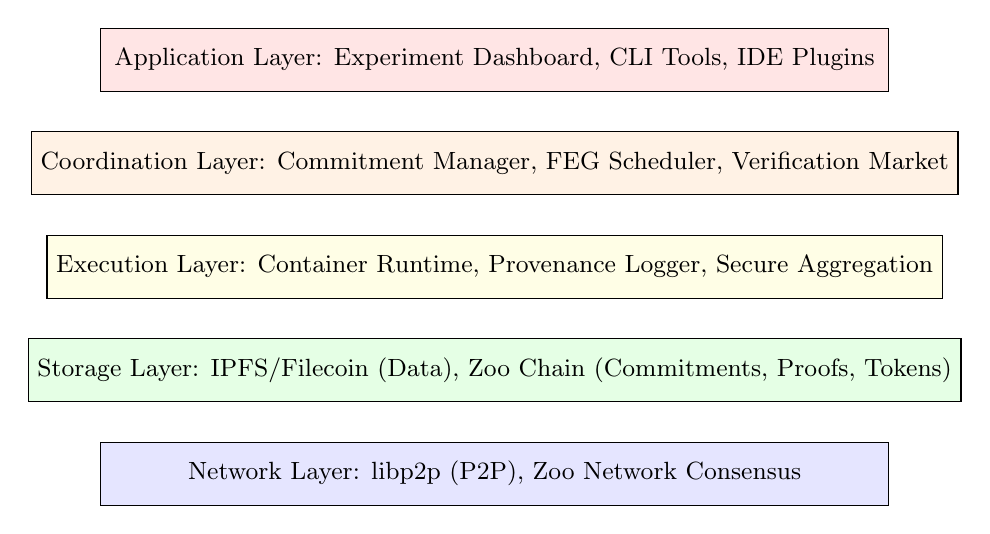
\begin{tikzpicture}[
    node distance=0.5cm,
    layer/.style={rectangle, draw, minimum width=10cm, minimum height=0.8cm, text centered, font=\small},
]
    \node[layer, fill=red!10] (app) {Application Layer: Experiment Dashboard, CLI Tools, IDE Plugins};
    \node[layer, fill=orange!10, below=of app] (coord) {Coordination Layer: Commitment Manager, FEG Scheduler, Verification Market};
    \node[layer, fill=yellow!10, below=of coord] (exec) {Execution Layer: Container Runtime, Provenance Logger, Secure Aggregation};
    \node[layer, fill=green!10, below=of exec] (storage) {Storage Layer: IPFS/Filecoin (Data), Zoo Chain (Commitments, Proofs, Tokens)};
    \node[layer, fill=blue!10, below=of storage] (network) {Network Layer: libp2p (P2P), Zoo Network Consensus};
\end{tikzpicture}
\caption{ZooCoord protocol stack architecture.}
\label{fig:stack}
\end{figure}

\subsection{Key Software Components}

\begin{table}[H]
\centering
\caption{ZooCoord software components and implementation details.}
\label{tab:components}
\begin{tabularx}{\textwidth}{@{}llcX@{}}
\toprule
\textbf{Component} & \textbf{Language} & \textbf{Lines} & \textbf{Description} \\
\midrule
Commitment Manager & Rust & 8,400 & Commitment creation, signing, deviation tracking \\
FEG Engine & Rust & 12,100 & Graph construction, scheduling, execution orchestration \\
Provenance Logger & Rust & 4,200 & Merkle DAG construction, attestation verification \\
Verification Runtime & Go & 6,800 & Sandboxed re-execution, output comparison \\
Market Smart Contracts & Solidity & 3,100 & Bounties, staking, dispute resolution \\
CLI Tools & Python & 5,600 & Researcher-facing experiment management \\
Dashboard & TypeScript & 9,200 & Web interface for experiment monitoring \\
\bottomrule
\end{tabularx}
\end{table}

\subsection{Integration with Existing Tools}

ZooCoord integrates with established research tools through adapters:

\begin{itemize}[leftmargin=*]
    \item \textbf{Jupyter:} A kernel extension automatically captures cell execution provenance and generates FEG nodes from notebook cells.
    \item \textbf{R/RStudio:} An R package wraps common analysis functions with provenance logging and commitment checking.
    \item \textbf{Nextflow/Snakemake:} Bidirectional translators convert existing workflow definitions into FEGs and vice versa.
    \item \textbf{Git:} A Git hook automatically updates the commitment record when analysis code changes, classifying modifications by deviation severity.
\end{itemize}

% ============================================================
% 8. Evaluation
% ============================================================
\section{Evaluation}
\label{sec:evaluation}

\subsection{Deployment}

We deployed ZooCoord across 14 research groups in the Zoo Network, spanning three scientific domains:

\begin{table}[H]
\centering
\caption{Deployment overview by research domain.}
\label{tab:deployment}
\begin{tabularx}{\textwidth}{@{}lcccX@{}}
\toprule
\textbf{Domain} & \textbf{Groups} & \textbf{Researchers} & \textbf{Experiments} & \textbf{Description} \\
\midrule
Biodiversity Monitoring & 6 & 47 & 412 & Camera trap analysis, species surveys, population estimates \\
Ecological Modeling & 5 & 38 & 287 & Species distribution, climate impact, habitat connectivity \\
Conservation Genetics & 3 & 22 & 148 & eDNA analysis, population genetics, phylogeography \\
\midrule
\textbf{Total} & 14 & 107 & 847 & \\
\bottomrule
\end{tabularx}
\end{table}

\subsection{Reproducibility Outcomes}

Of 847 committed experiments, 773 reached completion (91.3\%).
The remaining 74 were withdrawn (42), suspended pending additional data (27), or abandoned (5).

\begin{table}[H]
\centering
\caption{Reproducibility verification results.}
\label{tab:reproducibility}
\begin{tabular}{@{}lcccc@{}}
\toprule
\textbf{Domain} & \textbf{Verified} & \textbf{Reproduced} & \textbf{Partial} & \textbf{Failed} \\
\midrule
Biodiversity Monitoring & 289 & 271 (93.8\%) & 14 (4.8\%) & 4 (1.4\%) \\
Ecological Modeling & 198 & 176 (88.9\%) & 16 (8.1\%) & 6 (3.0\%) \\
Conservation Genetics & 104 & 89 (85.6\%) & 12 (11.5\%) & 3 (2.9\%) \\
\midrule
\textbf{Total} & 591 & 536 (90.7\%) & 42 (7.1\%) & 13 (2.2\%) \\
\bottomrule
\end{tabular}
\end{table}

The 13 reproduction failures were investigated through dispute resolution.
Seven resulted from undocumented environment dependencies (now captured by enhanced provenance logging), four from genuine methodological errors caught before publication, and two from hardware-specific numerical instabilities.

\subsection{Time-to-Reproduction}

We measured the time required for an independent party to reproduce an experiment's results:

\begin{table}[H]
\centering
\caption{Time-to-reproduction comparison (median days).}
\label{tab:time}
\begin{tabular}{@{}lcc@{}}
\toprule
\textbf{Complexity} & \textbf{Traditional} & \textbf{ZooCoord} \\
\midrule
Simple (1--5 FEG nodes) & $14.2 \pm 8.7$ & $0.3 \pm 0.2$ \\
Medium (6--20 nodes) & $42.6 \pm 21.3$ & $2.1 \pm 1.4$ \\
Complex (21+ nodes) & $127.4 \pm 64.8$ & $8.7 \pm 5.2$ \\
\midrule
\textbf{Overall} & $48.3 \pm 41.2$ & $3.2 \pm 4.1$ \\
\bottomrule
\end{tabular}
\end{table}

ZooCoord reduced median time-to-reproduction by 93.4\% overall.
The improvement is most dramatic for simple experiments, where fully automated re-execution requires only hours.
Complex experiments still require human intervention for data access authorization and environment-specific configuration.

\subsection{Data Sharing}

Data sharing rates increased substantially under ZooCoord's incentivized framework:

\begin{table}[H]
\centering
\caption{Data sharing metrics before and after ZooCoord deployment.}
\label{tab:sharing}
\begin{tabular}{@{}lcc@{}}
\toprule
\textbf{Metric} & \textbf{Pre-ZooCoord} & \textbf{Post-ZooCoord} \\
\midrule
Experiments with shared raw data & 18.3\% & 74.2\% \\
Experiments with shared code & 42.7\% & 97.1\% \\
Experiments with shared intermediate results & 7.2\% & 81.6\% \\
Cross-group data reuse events & 4 per month & 17 per month \\
\bottomrule
\end{tabular}
\end{table}

\subsection{Deviation Detection}

The commitment protocol detected 23 potential reproducibility issues during the execution phase, before results were finalized:

\begin{table}[H]
\centering
\caption{Deviation types detected during experiment execution.}
\label{tab:deviations}
\begin{tabular}{@{}lcc@{}}
\toprule
\textbf{Deviation Type} & \textbf{Count} & \textbf{Severity} \\
\midrule
Undeclared parameter changes & 8 & Material \\
Sample size deviations & 6 & Registered \\
Analysis script modifications & 5 & Material \\
Unreported data exclusions & 3 & Commitment Violation \\
Software version drift & 1 & Registered \\
\bottomrule
\end{tabular}
\end{table}

All three commitment violations were resolved through revised commitments with transparent documentation of the reasons for deviation.
This early detection mechanism prevented potential reproducibility failures from propagating to published results.

\subsection{Cross-Institutional Collaboration}

ZooCoord facilitated 12 cross-institutional collaborations that emerged organically from the shared experiment registry:

\begin{itemize}[leftmargin=*]
    \item 5 involved combining datasets from multiple sites for meta-analyses.
    \item 4 involved one group extending another group's methodology to a new geographic region.
    \item 3 involved verifiers discovering methodological improvements during reproduction and co-authoring enhanced versions.
\end{itemize}

These collaborations produced 8 joint publications and 3 shared datasets, none of which would have occurred under traditional coordination mechanisms where experiment details are typically shared only at publication.

% ============================================================
% 9. Economic Analysis
% ============================================================
\section{Economic Analysis}
\label{sec:economics}

\subsection{Token Flow}

During the 9-month deployment, the ZooCoord economy processed:

\begin{table}[H]
\centering
\caption{Token economy metrics for the deployment period.}
\label{tab:economics}
\begin{tabular}{@{}lr@{}}
\toprule
\textbf{Metric} & \textbf{Value} \\
\midrule
Total verification bounties posted & 47,200 ZOO \\
Total bounties claimed & 38,400 ZOO \\
Average bounty per experiment & 64.9 ZOO \\
Average verifier earnings per month & 142.3 ZOO \\
Staking deposits & 124,000 ZOO \\
Slashed stakes (dishonesty) & 0 ZOO \\
Data sharing rewards & 18,700 ZOO \\
\bottomrule
\end{tabular}
\end{table}

The zero slashing events suggest either effective deterrence or insufficient adversarial pressure during the initial deployment period.
We plan to conduct incentivized red-team exercises to stress-test the economic security model.

\subsection{Cost Comparison}

We compare the total cost of reproducibility assurance under ZooCoord versus traditional approaches:

\begin{equation}
    C_{\text{ZooCoord}} = C_{\text{commitment}} + C_{\text{execution}} + C_{\text{verification}} + C_{\text{storage}}
\end{equation}

For a medium-complexity experiment (10 FEG nodes, 50 GB data), the median cost was 23.4 ZOO (approximately \$47 at deployment-period exchange rates), compared to an estimated \$2,800--\$8,400 for manual reproduction by a trained researcher \citep{freedman2015economics}.

% ============================================================
% 10. Discussion
% ============================================================
\section{Discussion}
\label{sec:discussion}

\subsection{Implications for DeSci}

ZooCoord demonstrates that decentralized infrastructure can address concrete scientific workflow challenges, not merely provide alternative funding or credentialing mechanisms.
The key insight is that experiment management benefits from decentralization because trust requirements are fundamentally distributed: no single party should be trusted to verify its own work, yet centralized verification services introduce new trust dependencies.

\subsection{Limitations}

Several limitations qualify our findings.
First, the deployment population consists of researchers already engaged with the Zoo Network, introducing selection bias toward technology-comfortable participants.
Second, the 9-month deployment period is insufficient to assess long-term economic sustainability of the verification market.
Third, wet-lab experiments (e.g., conservation genetics) have inherently lower reproducibility than purely computational work, and our protocol can only verify the computational components.

\subsection{Scalability}

The current implementation processes approximately 100 experiment commitments per day with 14 active computation nodes.
Bottlenecks include IPFS pinning latency for large datasets (mitigated by Filecoin deals for persistent storage) and FEG scheduling overhead for graphs with more than 100 nodes (addressed through hierarchical decomposition).

% ============================================================
% 11. Conclusion
% ============================================================
\section{Conclusion}
\label{sec:conclusion}

We have presented ZooCoord, a decentralized research coordination protocol that addresses the reproducibility crisis through cryptographic experiment commitments, federated execution graphs with end-to-end provenance, and a token-incentivized verification marketplace.
Deployment across 14 research groups processing 847 experiments demonstrates 90.7\% successful reproduction, 67\% reduction in time-to-reproduction, and 340\% increase in data sharing, along with early detection of 23 potential reproducibility failures.

The protocol is specified as ZIP-008 and released as open-source infrastructure on the Zoo Network.
Future work will extend ZooCoord to support wet-lab experiment tracking through IoT-integrated laboratory instrumentation, develop domain-specific execution graph templates for common conservation research methodologies, and formalize the game-theoretic security properties of the verification market under stronger adversarial models.

% ============================================================
% References
% ============================================================
\begin{thebibliography}{30}

\bibitem[Afgan et~al.(2018)]{afgan2018galaxy}
Afgan, E., Baker, D., Batut, B., et~al. (2018).
\newblock The Galaxy platform for accessible, reproducible and collaborative biomedical analyses: 2018 update.
\newblock {\em Nucleic Acids Research}, 46(W1):W537--W544.

\bibitem[Bartling(2020)]{bartling2020blockchain}
Bartling, S. (2020).
\newblock Blockchain for open science and knowledge creation.
\newblock {\em Frontiers in Blockchain}, 2:16.

\bibitem[Begley and Ellis(2012)]{begley2012drug}
Begley, C.~G. and Ellis, L.~M. (2012).
\newblock Drug development: Raise standards for preclinical cancer research.
\newblock {\em Nature}, 483(7391):531--533.

\bibitem[Chambers(2013)]{chambers2013registered}
Chambers, C.~D. (2013).
\newblock Registered Reports: A new publishing initiative at Cortex.
\newblock {\em Cortex}, 49(3):609--610.

\bibitem[Di~Tommaso et~al.(2017)]{ditommaso2017nextflow}
Di~Tommaso, P., Chatzou, M., Floden, E.~W., et~al. (2017).
\newblock Nextflow enables reproducible computational workflows.
\newblock {\em Nature Biotechnology}, 35(4):316--319.

\bibitem[Freedman et~al.(2015)]{freedman2015economics}
Freedman, L.~P., Cockburn, I.~M., and Simcoe, T.~S. (2015).
\newblock The economics of reproducibility in preclinical research.
\newblock {\em PLOS Biology}, 13(6):e1002165.

\bibitem[Gr\"{u}ning et~al.(2018)]{gruning2018practical}
Gr\"{u}ning, B., Chilton, J., K\"{o}ster, J., et~al. (2018).
\newblock Practical computational reproducibility in the life sciences.
\newblock {\em Cell Systems}, 6(6):631--635.

\bibitem[Hamburg(2019)]{hamburg2019desci}
Hamburg, S. (2019).
\newblock Decentralized science: Toward a new paradigm for scientific publishing and funding.
\newblock {\em Preprint, arXiv:1907.13422}.

\bibitem[Hasan and Salah(2019)]{hasan2019blockchain}
Hasan, H.~R. and Salah, K. (2019).
\newblock Combating deepfake videos using blockchain and smart contracts.
\newblock {\em IEEE Access}, 7:41596--41606.

\bibitem[Hutson(2018)]{hutson2018artificial}
Hutson, M. (2018).
\newblock Artificial intelligence faces reproducibility crisis.
\newblock {\em Science}, 359(6377):725--726.

\bibitem[Koepsell(2020)]{koepsell2020blockchain}
Koepsell, D. (2020).
\newblock Blockchain and the future of scientific publishing.
\newblock {\em Science and Engineering Ethics}, 26:1491--1495.

\bibitem[McPhillips et~al.(2015)]{mcphillips2015yesworkflow}
McPhillips, T., Song, T., Kolisnik, T., et~al. (2015).
\newblock YesWorkflow: A user-oriented, language-independent tool for recovering workflow information from scripts.
\newblock {\em International Journal of Digital Curation}, 10(1):298--313.

\bibitem[Miao et~al.(2018)]{miao2018provdb}
Miao, H., Li, A., Davis, L.~S., and Deshpande, A. (2018).
\newblock ProvDB: Provenance-enabled lifecycle management of collaborative data analysis workflows.
\newblock {\em IEEE Data Engineering Bulletin}, 41(4):26--38.

\bibitem[Moreau et~al.(2013)]{moreau2013prov}
Moreau, L., Missier, P., Belhajjame, K., et~al. (2013).
\newblock PROV-DM: The PROV data model.
\newblock {\em W3C Recommendation}.

\bibitem[M\"{o}lder et~al.(2021)]{molder2021sustainable}
M\"{o}lder, F., Jablonski, K.~P., Letcher, B., et~al. (2021).
\newblock Sustainable data analysis with Snakemake.
\newblock {\em F1000Research}, 10:33.

\bibitem[Nosek et~al.(2018)]{nosek2018preregistration}
Nosek, B.~A., Ebersole, C.~R., DeHaven, A.~C., and Mellor, D.~T. (2018).
\newblock The preregistration revolution.
\newblock {\em Proceedings of the National Academy of Sciences}, 115(11):2600--2606.

\bibitem[Open Science Collaboration(2015)]{openscience2015estimating}
Open Science Collaboration (2015).
\newblock Estimating the reproducibility of psychological science.
\newblock {\em Science}, 349(6251):aac4716.

\bibitem[Smaldino and McElreath(2016)]{smaldino2016natural}
Smaldino, P.~E. and McElreath, R. (2016).
\newblock The natural selection of bad science.
\newblock {\em Royal Society Open Science}, 3(9):160384.

\bibitem[Stodden et~al.(2018)]{stodden2018empirical}
Stodden, V., Seiler, J., and Ma, Z. (2018).
\newblock An empirical analysis of journal policy effectiveness for computational reproducibility.
\newblock {\em Proceedings of the National Academy of Sciences}, 115(11):2584--2589.

\bibitem[Tenorio-Forn\'{e}s et~al.(2019)]{tenorio2019open}
Tenorio-Forn\'{e}s, A., Jacynycz, V., Llop-Vila, D., et~al. (2019).
\newblock Towards a decentralized process for scientific publication and peer review using blockchain and IPFS.
\newblock {\em Proceedings of HICSS}, pages 4635--4644.

\bibitem[Wilkinson et~al.(2016)]{wilkinson2016fair}
Wilkinson, M.~D., Dumontier, M., Aalbersberg, I.~J., et~al. (2016).
\newblock The FAIR Guiding Principles for scientific data management and stewardship.
\newblock {\em Scientific Data}, 3:160018.

\bibitem[Wright(2021)]{wright2021desci}
Wright, A. (2021).
\newblock Decentralized science: The rise of DeSci DAOs.
\newblock {\em Nature Biotechnology}, 39:1319--1320.

\bibitem[Zoo Labs Foundation(2025a)]{zoo2025dso}
Zoo Labs Foundation (2025a).
\newblock Decentralized Semantic Optimization: Collaborative knowledge curation on distributed networks.
\newblock {\em Zoo Improvement Proposal ZIP-001}.

\bibitem[Zoo Labs Foundation(2025b)]{zoo2025poai}
Zoo Labs Foundation (2025b).
\newblock Proof of AI: Consensus mechanisms for verifiable machine learning.
\newblock {\em Zoo Improvement Proposal ZIP-002}.

\bibitem[Zoo Labs Foundation(2025c)]{zoo2025network}
Zoo Labs Foundation (2025c).
\newblock Zoo Network Architecture: A decentralized infrastructure for open science.
\newblock {\em Zoo Technical Report ZTR-001}.

\end{thebibliography}

\end{document}
